\EnglishSourceFrame{GELFAND-P001485}{87}

\begin{equation*}
\int \mathcal{D}x\,e^{mL}
\longrightarrow
\int \mathcal{D}x\,\mathcal{D}\lambda\,
e^{\int \lambda^{-1}\dot{x}^{2}\,dt+\int m\lambda\,dt}
\tag{10}
\end{equation*}
[Before $m\lambda\,dt$, crossed out:
\EnglishUnclear{GELFAND-P001485}{eq10-cancellation}{an illegible sign, possibly $m$}.]

$L$ is as in (5)

Integrating the right-hand side by steepest descent (over $\lambda$), we obtain
$\lambda^{2}=\dfrac{\dot{x}^{2}}{m^{2}}$.

\begin{equation*}
\int \mathcal{D}x\,e^{m\int\sqrt{\dot{x}^{2}}\,dx}
\tag{11}
\end{equation*}
\EnglishUnclear{GELFAND-P001485}{eq11-differential}{At the end of the exponent: $dx$; possibly $dt$.}

((11) $\Rightarrow$ (10) gets rid of the square root). It turns out that the equality is exact!!

The number $\lambda$ has the meaning of a 1-dimensional metric
(all the rest \EnglishUnclear{GELFAND-P001485}{metric-abbreviation}{reduc. / free [source abbreviations]}
from reparametrization)

\begin{equation*}
\int\frac{d\lambda}{\lambda}\,e^{a\lambda}e^{b/\lambda}
=e^{\sqrt{ab}}
\tag{12}
\end{equation*}
\EnglishUnclear{GELFAND-P001485}{eq12-identity}{The equality has $e^{\sqrt{ab}}$ with no further factors.}

Green and others did an analogous thing in string theory: passing to

\begin{equation*}
\sum_{\text{topol.}}\int\mathcal{D}x\,\mathcal{D}g\,
e^{\int\sqrt{g}\,g^{ab}\partial_a x^{\mu}\partial_b x^{\mu}\,d\sigma\,dt}
\underbrace{e^{\int\sqrt{g}\,d\sigma\,dt}}_{\text{this can be omitted}}
\tag{13}
\end{equation*}

\underline{Generalization:}

curved 26-dimensional space

\begin{equation*}
\begin{aligned}
\sum_{\text{topol.}}\int\mathcal{D}x\,\mathcal{D}g\,
e^{\int G_{\mu\nu}(x)\sqrt{g}\,g^{ab}\partial_a x^{\mu}\partial_b x^{\nu}}
&{}\\
&d\sigma\,dt
\end{aligned}
\tag{14}
\end{equation*}
\EnglishUnclear{GELFAND-P001485}{eq14-differentials}{The factor $d\sigma\,dt$ is written below the exponent; whether it belongs inside the exponent is unclear.}

We want Einstein's equations to hold

\begin{equation*}
R_{\mu\nu}(x)=0
\tag{15}
\end{equation*}

\begin{equation*}
\begin{gathered}
(15)\ \Leftrightarrow\ \text{dilatational invariance!}\\
\Downarrow\\
\text{Yang--Mills eqs.}
\end{gathered}
\end{equation*}

All invariant equations for higher fields follow from dilatational
invariance (in the one-loop approximation)

\EnglishSourceFrame{GELFAND-P001486}{unlabelled}

\underline{$26/\overline{\underline{\mathrm{IX}}}$-88 yr.}
\qquad \underline{\underline{Gelfand's sem.}}

\underline{I.M.G.} Read Feynman's book on QED and
\EnglishUnclear{GELFAND-P001486}{feynman-verb}{learn / learn [imperative plural] / learn for oneself}
\EnglishUnclear{GELFAND-P001486}{feynman-noun}{aesthetics [two source case endings]}
from him.

There QED is presented without formulas, using pictures alone.

\underline{\underline{Kazakov.}}
\quad \underline{Combinatorics and new work on strings}

Developments have occurred (in combinatorics)

\underline{Polyakov} and
[crossed out: \EnglishUnclear{GELFAND-P001486}{names-cancellation}{po? [source letters]}]
\underline{Zamolodchikov --- Knizhnik --- Polyakov}
showed that the models presented above do indeed describe 2-dimensional
quantum gravity.

(Knizhnik --- Polyakov --- Zamolodchikov)

[Below the names:] in English alphabetical order.

Z.-K.-P. considered a bosonic string model.

\begin{equation*}
S=\int d^{2}\xi\,\sqrt{g}\,\partial_a x^{\mu}\partial_b x^{\mu}\,g^{ab}
+\beta\int d^{2}\xi\,\sqrt{g}
\tag{1}
\end{equation*}

\begin{equation*}
Z(\beta)=\int\mathcal{D}g_{ab}\int\mathcal{D}x^{\mu}\,e^{-S}
\tag{2}
\end{equation*}

$\mu=1,\ldots,D$.

\EnglishSourceFigure{GELFAND-P001486}{metric-diagram}{At the lower right are two approximately perpendicular intersecting axes: the horizontal one labeled $\xi_1$ on the right, the vertical one labeled $\xi_2$ at the upper left. To the right of the vertical axis and above the horizontal is a closed irregular outline containing $g_{ab}(\xi)$. The directions of the axis arrowheads cannot confidently be distinguished.}

\par\medskip\noindent
\begin{minipage}[c]{0.48\linewidth}\centering
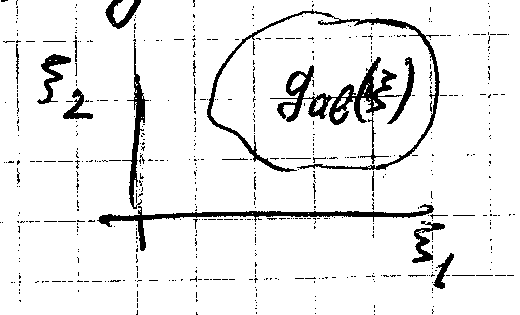
\includegraphics[width=\linewidth]{figures/gelfand-p001486-metric-diagram-original.png}
\par\smallskip{\footnotesize Original manuscript diagram: GELFAND-P001486\par}
\end{minipage}\hfill
\begin{minipage}[c]{0.48\linewidth}\centering
\resizebox{\linewidth}{!}{% Partial visible-stroke recreation. Endpoint hooks do not assert arrows; gaps remain open.
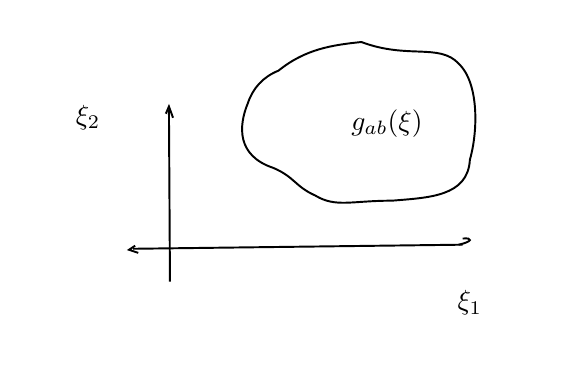
\begin{tikzpicture}[x=0.013cm,y=-0.013cm,line width=0.7pt]
\path[use as bounding box] (0,0) rectangle (520,315);
\draw (139,248)--(138,80);\draw (135,84)--(138,77)--(142,88);
\draw (103,216)--(425,212);\draw (105,213)--(99,217)--(108,220);
\draw (421,212)..controls(435,209)and(435,205)..(425,206);
\draw (245,42)..controls(271,21)and(297,17)..(326,14)
 ..controls(371,31)and(402,15)..(421,35)
 ..controls(441,54)and(440,101)..(432,129)
 ..controls(430,165)and(392,166)..(356,169)
 ..controls(316,169)and(301,176)..(281,164)
 ..controls(261,155)and(261,146)..(240,137)
 ..controls(204,125)and(206,96)..(215,74)
 ..controls(220,59)and(230,48)..(245,42);
\node at (59,88) {$\xi_2$};\node at (432,269) {$\xi_1$};
\node at (351,94) {$g_{ab}(\xi)$};
\end{tikzpicture}
}
\par\smallskip{\footnotesize Partial recreation; uncertain directions and joins remain unresolved.\par}
\end{minipage}\par\medskip


\EnglishSourceFrame{GELFAND-P001487}{unlabelled}

The integral (2) is defined for
\EnglishUnclear{GELFAND-P001487}{top-beta-inequality}{$\beta>\beta_c$ / $\beta\ge\beta_c$; the sign is corrected}
and behaves there as
\begin{equation*}
(\beta-\beta_c)^{2-\gamma_{\mathrm{str}}(D)}
\tag{3}
\end{equation*}

(at $\beta_c$, the surface volume becomes infinite)

[Above the line: $\mathrm{str}=\mathrm{string}$.]

K.-P.-Z. proved that
\begin{equation*}
\gamma_{\mathrm{str}}=\frac{1}{12}
\left(D-1-\sqrt{(D-1)(D-25)}\right).
\tag{4}
\end{equation*}

This makes sense for
\EnglishUnclear{GELFAND-P001487}{upper-dimension-range}{$D\le1$ and $D\ge26$ [as in the source]}.
This was obtained using Kac--Moody algebras that arose in studying
the Lagrangian.

\underline{Kazakov and others} predicted several values of $\gamma_{\mathrm{str}}$:
for $D=-2,0,\frac12,1$

[In the left margin:
\EnglishUnclear{GELFAND-P001487}{left-margin-monogram}{IG / IM? [source initials]}.]
Everything agreed!!

Define:
\begin{equation*}
Z(\beta)=\sum_{n=0}^{\infty}e^{-2n\beta}Z_{2n},
\tag{5}
\end{equation*}
where $Z_n$ is the number of planar graphs
[inserted above the line: with $n$ vertices]
with the topology of the sphere
(3 edges must meet at a vertex)

Then
\begin{equation*}
Z(\beta)\sim(\beta-\beta_c)^{2-\gamma_{\mathrm{str}}(D)}
\tag{6}
\end{equation*}
[A bracket is drawn above $\gamma_{\mathrm{str}}(D)$; on its right: $=-\frac12$.]
This corresponds to $D=0$

\EnglishSourceFigure{GELFAND-P001487}{right-margin-triangle-graphs}{Two drawings are arranged vertically in the right margin. The upper drawing has a large triangle with an upper vertex and horizontal base, containing a smaller triangle with the same orientation. Each inner vertex joins the corresponding outer vertex. On the inner base near its left vertex is a thickening resembling a leftward arrowhead; by the outer lower-right vertex are strokes resembling a rightward arrowhead. The lower drawing has an outer triangle and three segments from its vertices toward an inner point; the segment from the lower-left vertex stops just short of the meeting point of the other two. Neither drawing has letter or number labels. The arrowheads and meaning of the lower gap require checking.}

\par\medskip\noindent
\begin{minipage}[c]{0.48\linewidth}\centering
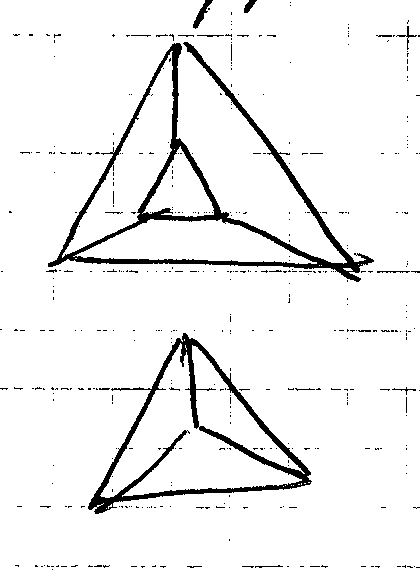
\includegraphics[width=\linewidth]{figures/gelfand-p001487-right-margin-triangle-graphs-original.png}
\par\smallskip{\footnotesize Original manuscript diagram: GELFAND-P001487\par}
\end{minipage}\hfill
\begin{minipage}[c]{0.48\linewidth}\centering
\resizebox{\linewidth}{!}{% Partial visible-stroke recreation. Endpoint hooks do not assert arrows; gaps remain open.
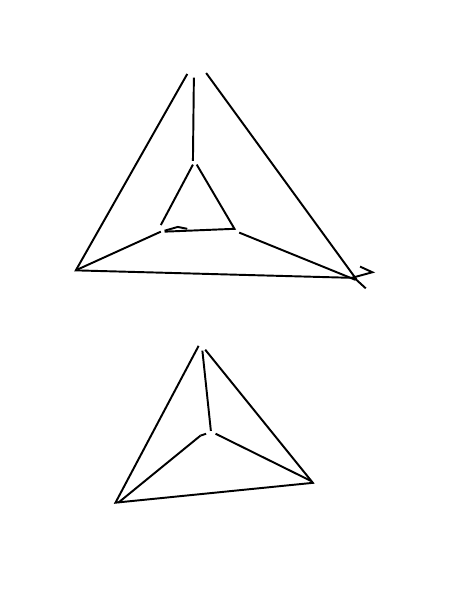
\begin{tikzpicture}[x=0.012cm,y=-0.012cm,line width=0.7pt]
\path[use as bounding box] (0,0) rectangle (420,570);
\draw (169,49)--(51,257)--(347,265)--(189,48);
\draw (176,53)--(175,141);\draw (175,145)--(141,209);
\draw (179,145)--(219,213)--(145,216);\draw (141,216)--(53,256);
\draw (224,217)--(347,267);\draw (145,215)--(159,211)--(169,213);
\draw (343,265)--(365,259)--(352,253);\draw (347,266)--(358,276);
\draw (181,337)--(93,503)--(302,482)--(188,341);
\draw (185,342)--(194,427);\draw (199,430)--(300,480);
\draw (96,503)--(183,432);\draw (183,432)--(189,430);
\end{tikzpicture}
}
\par\smallskip{\footnotesize Partial recreation; uncertain directions and joins remain unresolved.\par}
\end{minipage}\par\medskip


[Crossed out:
\EnglishUnclear{GELFAND-P001487}{middle-cancelled-word}{number?}.]
Asymptotics
\begin{equation*}
Z_{2n}\sim\left(\frac{256}{27}\right)^n n^{-3+\gamma_{\mathrm{str}}}
\tag{7}
\end{equation*}

$\gamma_{\mathrm{str}}$ is a universal number independent of the way planar graphs are defined
(one can have 4 edges at 1 vertex, etc.)

\underline{Formula for $Z_n$.}

[Before the retained right-hand side of (8), a fraction is crossed out:
\EnglishUnclear{GELFAND-P001487}{bottom-cancelled-fraction}{$2\frac{(4n+7)!}{(n-4)}$ / $2\frac{(4n+1)!}{(n-4)}$ / $2\frac{(4n-7)!}{(n-4)}$; $n$ or $k$, and the denominator factorial is unclear}.]
\begin{equation*}
Z_{2k}=2\frac{(4k-3)!}{(3k-1)!\,k!}
\tag{8}
\end{equation*}
[On the right in (8) is the factor:
\EnglishUnclear{GELFAND-P001487}{bottom-final-factor}{$9^k$ / $g^k$}.]

$Z_{2k}$ is the number of planar graphs inscribed in a triangle ($\Delta$), with
the number of inner vertices $=2k$.

\EnglishSourceFrame{GELFAND-P001488}{91}

Tutte solved this problem purely combinatorially.

\EnglishSourceFigure{GELFAND-P001488}{top-triangle-graph}{At the upper left is an outer triangle with an upper vertex and almost horizontal base. Inside is a smaller triangle labeled 1 by its upper vertex, $i$ by its lower-left vertex and 2 by its lower-right vertex. Corresponding outer and inner vertices are joined; the edge between inner vertices 1 and 2 is curved. On the left outer edge is a thickening resembling a downward arrowhead. It is unclear whether this denotes an arrow or an overlap of strokes.}

\par\medskip\noindent
\begin{minipage}[c]{0.48\linewidth}\centering
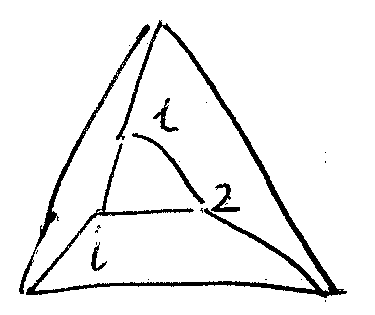
\includegraphics[width=\linewidth]{figures/gelfand-p001488-top-triangle-graph-original.png}
\par\smallskip{\footnotesize Original manuscript diagram: GELFAND-P001488\par}
\end{minipage}\hfill
\begin{minipage}[c]{0.48\linewidth}\centering
\resizebox{\linewidth}{!}{% Partial visible-stroke recreation. Endpoint hooks do not assert arrows; gaps remain open.
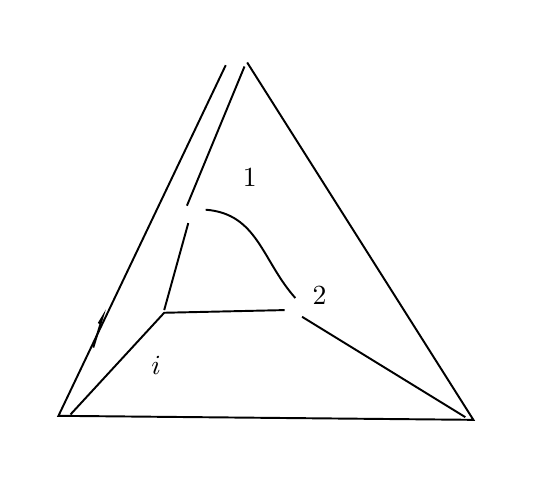
\begin{tikzpicture}[x=0.017cm,y=-0.017cm,line width=0.7pt]
\path[use as bounding box] (0,0) rectangle (375,315);
\draw (148,28)--(23,290)--(333,293)--(164,26);
\draw (162,29)--(119,133);\draw (120,146)--(102,211);
\draw (32,289)--(102,213)--(192,211);
\draw (133,136)..controls(172,139)and(175,174)..(200,202);
\draw (205,216)--(327,291);\draw (49,239)--(56,216)--(53,221);
\node at (166,112) {$1$};\node at (96,252) {$i$};\node at (218,200) {$2$};
\end{tikzpicture}
}
\par\smallskip{\footnotesize Partial recreation; uncertain directions and joins remain unresolved.\par}
\end{minipage}\par\medskip


Consider
\begin{equation*}
Z_n=\sum_{\substack{\text{graphs}\\ \text{with }n\\ \text{vert.}}}
\int\prod_{i=1}^{n}d\vec{x}_i\,
e^{-\sum_{\langle ij\rangle}(x_i^{\mu}-x_j^{\mu})^2}
\tag{9}
\end{equation*}

$\langle ij\rangle$ are nearest neighbors in the graph;

inner vertices

(10) The integral in (9) equals $\det^{-D/2}(3I-G)$.

[A stroke leads from $G$ to the explanation:]
Matrix of [crossed out:
\EnglishUnclear{GELFAND-P001488}{middle-cancelled-incidence}{incidence?}]
vertex adjacency

($G_{ij}=1\Longleftrightarrow i,j$ are joined by an edge

$G_{ij}=0$
\EnglishUnclear{GELFAND-P001488}{middle-overdrawn-equivalence}{a densely retraced / crossed-out sign $\Longleftrightarrow$}
otherwise).

[In the first line, $G$ is corrected:
\EnglishUnclear{GELFAND-P001488}{middle-overdrawn-matrix-symbol}{the earlier sign $E$ / $G$?}.]

\underline{\underline{Kapranov Misha.}}

\underline{On work [crossed out: B.-G.-G.] on $\mathcal{D}$-modules.}
[Inserted below the cancelled abbreviation: Bernsht.-Gelf.-Gelf.]

$V$ is a vector [crossed out:
\EnglishUnclear{GELFAND-P001488}{lower-cancelled-space-token}{pr / an illegible short sign}]
space, $P(V)$ is its projectivization.

$O(-1)$ is a bundle on $P(V)$ (the basic one);
[inserted above “bundle”: tautological]

[On the right:]
\begin{equation*}
O(-1)\subset P(V)\times V
\end{equation*}
[Below $O(-1)$:
\EnglishUnclear{GELFAND-P001488}{lower-tautological-annotation}{two vertical curved strokes: a vertical equality / a double mark?},
to their right $\{(\ell,x)\mid x\in\ell\}$.]

The points of $P(V)$ are lines $\ell$ in $V$ through $0$;
the line is the fiber over $\ell$.

$O(-k)=O(-1)^{\otimes k}$, $k>0$;

$O(+k)$ is the bundle dual to $O(-k)$.

\underline{A way of constructing new bundles:}

$\Lambda(V)$ is the exterior algebra on $V$;

$\Lambda^k(V)$ is the homogeneous degree-$k$ part of $\Lambda(V)$.

Consider graded modules over $\Lambda(V)$.
\begin{equation*}
\{\ldots\ M_{-1};\ M_0;\ M_1;\ \ldots\},
\qquad \Lambda^kM_i\subset M_{i+k}.
\end{equation*}

\underline{Exercise for next time:} write down the answers for
[crossed out:
\EnglishUnclear{GELFAND-P001488}{bottom-cancelled-exercise-symbol}{$M$ / $V$?}]
$\dim V=1$ and $2$.

\EnglishSourceFrame{GELFAND-P001489}{unlabelled}
$V\ni v$, $v^2=0$ in $\Lambda(V)$.

Consider multiplication by $v$:
\begin{equation*}
(1)\qquad
\ldots\to M_{-1}\overset{v}{\longrightarrow}M_0
\overset{v}{\longrightarrow}M_1\overset{v}{\longrightarrow}M_2\to\ldots
\end{equation*}
$v^2=0\ \Rightarrow$ this gives a complex.
\begin{equation*}
\operatorname{Ker}v\supset\operatorname{Im}v,
\end{equation*}
[Crossed out to the right of the formula:
\EnglishIncomplete{GELFAND-P001489}{cancel-after-image}{The crossed-out fragment cannot be read.}]

Consider [crossed out:
\EnglishIncomplete{GELFAND-P001489}{cancel-before-bundle}{The crossed-out fragment between “Consider” and “bundle” cannot be read.}]
the bundle
\begin{equation*}
v\longmapsto
\frac{\operatorname{Ker}\{v:M_0\to M_1\}}
{\operatorname{Im}\{v:M_{-1}\to M_0\}},\qquad v\ne0.
\end{equation*}
This is a “bundle”, or more precisely a “sheaf”, on $\mathbb P(V)$.

\underline{Examples.}\newline
\underline{of modules}

1). $\Lambda(V)$ itself
\begin{equation*}
\underset{0}{\mathbb C}\overset{v}{\longrightarrow}
\underset{1}{V}\overset{v}{\longrightarrow}
\underset{2}{\Lambda^2V}\overset{v}{\longrightarrow}
\ldots\overset{v}{\longrightarrow}\underset{N}{\Lambda^NV}
\end{equation*}
It corresponds to the zero bundle; $\operatorname{Ker}v=\operatorname{Im}v$.

2) The truncated algebra $\Lambda$, i.e. $\Lambda^{\ge k}(V)$

(only components of degrees $\ge k$ are retained).
\begin{equation*}
\{0;\ \Lambda^kV\overset{v}{\longrightarrow}\Lambda^{k+1}V;\ \ldots\}
\end{equation*}
[A sign below the arrow is crossed out:
\EnglishUnclear{GELFAND-P001489}{truncated-arrow-cancel}{$v$ / $k$.}]

The bundle:
\begin{equation*}
\operatorname{Ker}\{v:\Lambda^kV\to\Lambda^{k+1}V\}
=\Omega^{k-1}_{\mathbb P(V)}\otimes O(k)
\end{equation*}
[A line beneath $\Omega^{k-1}_{\mathbb P(V)}$ leads to the caption:
$(k-1)$-forms on $\mathbb P(V)$.]

3) Let $V$ be a symplectic space, $[\ ,\ ]$ a $2$-form;
[above “$2$-form”, inserted and joined by a brace:
\EnglishUnclear{GELFAND-P001489}{symmetry-note}{symm.}]

consider the module
\begin{equation*}
0\to\underset{-1}{\mathbb C}\overset{v}{\longrightarrow}
\underset{0}{V}\overset{v}{\longrightarrow}\underset{1}{\mathbb C}\to0
\end{equation*}
\begin{equation*}
v:w\longmapsto[v,w]
\end{equation*}
\begin{equation*}
v\longmapsto v^{\perp}/\mathbb Cv,
\qquad\perp\text{ --- orthog. w.r.t. }[\cdot,\cdot]
\end{equation*}

\underline{Theorem.} Every algebraic vector bundle
on $\mathbb P(V)$ arises from some $\Lambda(V)$-module
\begin{equation*}
E=\frac{\operatorname{Ker}\{v:M_0\to M_1\}}
{\operatorname{Im}\{v:M_{-1}\to M_0\}},
\quad\text{and the other factors }=0.
\end{equation*}

\EnglishSourceFrame{GELFAND-P001490}{92}
\underline{Proof}: see S. Gelfand's appendix
to the book by \underline{Okonek} and others, “Bundles over project. space”.

\underline{Statement}: a note in FA in 1978.

The proof uses \underline{derived} categories. Can this
be avoided? S. Gelfand thinks not.

\underline{Kapranov's result}: a description of bundles on a quadric
in $\mathbb P(V)$.
\begin{equation*}
V,\quad\langle\ \rangle,\qquad
\mathbb P(V)\supset Q=\{v:\langle v,v\rangle=0\}
\end{equation*}
[A line from $\langle\ \rangle$ leads to the caption: symm. form.]

Construct the graded Clifford algebra [inserted above the line with a bracket: $A(V)$],
generated by
\begin{equation*}
v,\quad\operatorname{deg}v=1\text{ and }h,\quad\operatorname{deg}h=2
\end{equation*}
[A line from $h$ leads to the caption: fixed]
\begin{equation*}
vv'+v'v=\langle v,v'\rangle h
\end{equation*}
In an \EnglishUnclear{GELFAND-P001490}{basis-abbreviation}{orthon. / orthog.}
basis $e_1,\ldots,e_r$
\EnglishUnclear{GELFAND-P001490}{clifford-normalization}{$e_i^2=h,\qquad
e_ie_k=-e_ke_i,\quad i\ne k.$}
For $r=3$, this is $\approx$ quaternions.

\begin{equation*}
\langle v,v\rangle=0\ \Rightarrow\ v^2=0
\end{equation*}
and construct the same kind of bundle.

Then the same kind of theorem holds.

